\documentclass[12pt]{article}

\usepackage{amsmath}
\usepackage{amssymb}
\usepackage{graphicx}
\usepackage[outdir=./]{epstopdf}
\usepackage{setspace}
\usepackage{geometry}
\usepackage{booktabs}
\usepackage{hyperref}
\usepackage{xurl}
\usepackage{float}
\usepackage{makecell}
\usepackage[expansion=false]{microtype}
\geometry{margin=1in}
\setstretch{1.2}

\title{The Nonlinear Geometry of State-Building: \\Mapping Global Governance Trajectories via Manifold Learning}

\author{
Adriel I. Santoso \\
Department of Mechanical and Aerospace Engineering \\
Tohoku University
}

\date{\today}

\begin{document}

\maketitle

\begin{abstract}
    Comparative political science often relies on discrete regime types that assume state development follows linear paths. This paper instead treats global governance as a continuous dynamical system. Using longitudinal Quality of Government (QoG) data from 1990 to 2026, we construct a global governance phase-space using non-linear diffusion maps. We project decades of historical data onto a 2026 reference manifold using the Nyström approximation to reveal the latent structure of state-building.

    We introduce two new macro-political metrics, trajectory tortuosity and geodesic inefficiency, to help characterize patterns of institutional movement. Unsupervised clustering shows three distinct developmental patterns: direct, meandering, and erratic. These erratic paths often pass through low-density regions of the manifold, suggesting that rare regime configurations are fundamentally unstable. Furthermore, we find that past institutional displacement predicts future movement, which is consistent with path-dependent dynamics. Our results suggest that a state’s movement through the governance manifold offers more analytical insight than its static classification, challenging standard indicator-based frameworks.
\end{abstract}

\section{Introduction}

Following the Cold War, market liberalization and democratization were widely expected to drive global institutional convergence \cite{fukuyama1989end, fukuyama2011origins, carothers2002end}. The ensuing decades have defied these predictions by yielding persistent institutional divergence. Political science continues to measure this complex reality with largely static tools. Annual indicators sort states into typological bins, discarding the historical trajectory data necessary to distinguish a consolidating system from one nearing instability.

This information loss has concrete consequences. In Kyrgyzstan, for example, conventional metrics showed measurable progress in the early 2000s, which standard monitoring frameworks would have recorded as improvement. However, its trajectory revealed political liberalization sharply misaligned with underlying structural capacity. The subsequent periods of instability in 2005, 2010, and 2020 were not isolated anomalies. They were structurally prefigured by the state's passage through empirically unstable configurations, a dynamic that static indicators inherently obscure.

Viewing global governance as a complex adaptive system, this paper argues that a state's trajectory is far more informative than its static position \cite{miller2007complex, simon1962architecture}. States are dynamic entities navigating a structured landscape of institutional possibilities. Consequently, the central empirical question is not merely where a state currently sits, but how it has moved. It is essential to ask whether a state's path is directed and stable, or erratic and prone to configurations the global system rarely sustains.

To operationalize this, we apply Diffusion Maps to longitudinal Quality of Government data (1990–2026) to construct a global governance phase space that maps institutional co-variation across 166 countries. Within this nonlinear embedding, we introduce Trajectory Tortuosity and Geodesic Inefficiency as two novel macro-political metrics to quantify developmental paths. These metrics allow us to identify Direct, Meandering, and Erratic movement paradigms via unsupervised clustering. Finally, a dispersion analysis within this framework reveals that since 1992, the global governance distribution has continuously polarized into competing developmental basins rather than converging. By making this toolkit publicly available, we provide an empirical foundation for trajectory-aware theories of institutional change, enabling future research into the underlying causal mechanisms.

\section{Theoretical Context and Literature Review}

\subsection{The Limits of Discrete Typologies}
Comparative political science has long relied on discrete categorizations to measure state development. Indices such as Polity IV, Freedom House, and the Varieties of Democracy (V-Dem) project \cite{coppedge2025vdem} are routinely deployed to sort nations into taxonomic bins: ``closed autocracies,'' ``electoral autocracies,'' or ``consolidated democracies.'' These typologies are heuristically useful for descriptive statistics and panel regressions, yet they share a structural limitation: they represent a dynamic system as a static point, discarding the directional information encoded in how a state arrived at its current configuration.

The classical ``transition paradigm'' assumed that states move along a broadly linear continuum toward democratic consolidation and economic modernization \cite{huntington1991third}. Subsequent decades have complicated this expectation considerably. Democratic backsliding \cite{bermeo2016democratic}, stalled transitions, and a measurable third wave of autocratization \cite{lhrmann2019third} have each demonstrated that institutional change is not unidirectional, and that the same formal categorization can conceal radically different developmental logics. Two states may occupy the same ``electoral autocracy'' bin at the same moment, one consolidating bureaucratic capacity incrementally, the other reverting from a prior democratic peak, yet standard indicator-based methods offer no systematic way to distinguish them. The difficulty is not primarily one of measurement precision; it is that the spatial and temporal continuity of state-building falls outside the scope of cross-sectional scores by construction.

Several qualitative frameworks in the political science literature implicitly recognize this limitation. Linz and Stepan's \cite{linzstepan1996} theory of democratic consolidation distinguishes between transitions that are behaviorally, attitudinally, and constitutionally consolidated, a tripartite condition that can be satisfied at very different rates, producing states with identical formal classifications but radically different developmental momentum. Their framework implies that consolidation is a trajectory property rather than a threshold: what matters is whether institutional, civic, and constitutional dimensions are co-evolving or diverging from one another. This is precisely the distinction that static indicator scores cannot capture and that trajectory geometry is designed to recover.

Levitsky and Way's \cite{levitskyway2010} account of competitive authoritarianism sharpens the problem further. They document regimes that adopt the formal apparatus of democracy, multiparty elections, legislatures, nominally independent courts, without the organizational capacity or ruling-party cohesion required to make these institutions self-enforcing \cite{diamond2002elections, schedler2002menu}. The outcome is a class of states that score ambiguously on standard indices while following a characteristic trajectory: rapid movement into configurations where institutional form outpaces structural substance, followed by reversion toward more coherent arrangements. In the geometric framework developed here, this pattern corresponds to the Erratic typology, states repeatedly passing through low-density manifold regions that the broader cross-national distribution rarely sustains. The trajectory geometry provides Levitsky and Way's qualitative observation with a quantitative counterpart.

\subsection{State-Building as a Complex Adaptive System}
Moving beyond static categories requires a framework in which states are understood not as points to be classified but as dynamic entities navigating a structured landscape of institutional possibilities. This paper conceptualizes global governance as a complex adaptive system operating within a continuous mathematical space \cite{miller2007complex, simon1962architecture}. Countries are not isolated observations to be sorted into bins; they are trajectories through a multi-dimensional phase-space defined by their institutional, social, and economic parameters, and the shape of those trajectories carries information about the system's underlying dynamics.

This perspective aligns with recent advances in political economy that treat institutional development as highly non-linear. Most notably, Acemoglu and Robinson's concept of the ``Narrow Corridor'' \cite{acemoglu2019narrow, acemoglu2012why} posits that sustained development requires the co-evolution of state capacity and societal liberty in a delicate, precarious balance. Where state capacity outpaces societal control, the system is drawn toward despotic attractors; where societal fragmentation outpaces state capacity, it risks collapse into anarchic or deeply inefficient configurations. The corridor between these failure modes is not a fixed destination but a moving target, and the conditions required to remain within it are fundamentally relational rather than absolute.

\subsection{The Geometry of Governance}

Translating the Narrow Corridor into the language of differential geometry opens a new analytical register. The viable pathways for state development do not fill the entirety of the theoretical parameter space; they are constrained to a lower-dimensional manifold, a specific geometric surface embedded within the higher-dimensional data. This constraint is not imposed by the analyst; it reflects the empirical fact that not all combinations of institutional and economic indicators are simultaneously realized across the cross-national distribution.

By applying manifold learning to longitudinal cross-national data, this structure can be recovered directly from the data rather than assumed in advance. Rather than positing linear transition paths, the approach estimates the ``terrain'' of global governance empirically. Within this terrain, stable institutional arrangements function as attractors, while configurations in which institutional and structural variables are sharply misaligned tend to be rarely occupied, a property we describe as high-friction for convenience, without implying that friction operates as a causally identified force.

The high-density spine of the resulting manifold is not a geometric artifact; it is an empirical trace of the Narrow Corridor itself. Acemoglu and Robinson posit that the corridor occupies a precarious band in the joint space of state capacity and societal liberty, bounded by despotic over-reach on one side and anarchic fragmentation on the other \cite{acemoglu2019narrow}. In our embedding, Component 1 (Socio-Institutional Capacity, loading strongly on egalitarianism and corruption control) and Component 2 (Structural Modernization, loading on GDP and urbanization) jointly define a space in which the corridor corresponds to the region where institutional and structural development co-evolve at compatible rates. The low-density zones flanking the spine, where high structural wealth coexists with extreme corruption, or where rapid liberalization outpaces underlying state capacity, are precisely the configurations that states rarely sustain, because they lie outside the corridor. The diffusion manifold does not assume this structure; it recovers it from cross-national data. The correspondence between the manifold's density topology and the theoretical corridor thus constitutes an independent empirical check on Acemoglu and Robinson's framework, and motivates the interpretation of low-density regions as structurally unstable rather than merely statistically rare.

Evaluating a state's trajectory through this landscape makes it possible to measure not only its current position but the efficiency and coherence of its movement through the permissible pathways of institutional development.

\section{Methodology}

The analysis proceeds in two stages. In the first, we construct a low-dimensional embedding of the 2026 cross-section of governance configurations, using this as a reference manifold against which historical trajectories can be measured. In the second, we project longitudinal data from 1990 to 2026 onto this static reference and compute trajectory-level metrics from the resulting paths. Throughout, we treat the recovered geometry as a descriptive scaffold for characterizing patterns of institutional movement. Regions of low empirical density are interpreted as configurations that states rarely sustain, a property we term \textit{structural friction} for convenience, though this label reflects a geometric observation rather than a causally identified force.

\subsection{Data Acquisition and Preprocessing}
The empirical foundation is the Quality of Government (QoG) Standard Dataset, drawn on in two complementary forms: a cross-sectional slice for manifold construction, and time-series observations from 1990 to 2026 for trajectory projection \cite{teorell2026qog}. The post-1990 timeframe is chosen specifically to capture the institutional dynamics that followed the Cold War's end and the ``Third Wave'' of democratization.

We analyze state configurations across ten dimensions organized into four theoretically distinct blocks, detailed in \S\ref{subsec:varselect}. The baseline six span political institutions (V-Dem Electoral Democracy, Egalitarianism, and Corruption) and structural modernization (GDP per capita, Life Expectancy, Urbanization). Four variables extend the space into dimensions entirely absent from the baseline: Government Effectiveness (\textit{wbgi\_gee}) and Tax Revenue as a share of GDP (\textit{wdi\_taxrev}) operationalize state capacity; the Liberal Component (\textit{vdem\_liberal}) adds horizontal accountability and civil liberties; and Trade Openness (\textit{wdi\_trade}) captures external economic integration.

\subsection{Missing Data: A Political Representativeness Problem}

Missingness in global governance datasets is not random noise—it is a political signal. Authoritarian regimes, collapsing states, and internationally isolated governments systematically suppress or fail to report the indicators that international datasets depend on. In the QoG dataset used here, the 27 countries (of 194) that lack complete data on all six variables are disproportionately concentrated in the low-institutional-capacity region of the governance space: the configurations this paper is most analytically interested in. Listwise deletion of these cases would not produce a statistically cleaner sample; it would produce a politically truncated one, systematically excising the autocracy end of the manifold and biasing the embedding's geometry toward high-capacity, data-rich states.

Table~\ref{tab:missingness} documents this pattern directly. Countries with at least one missing value across the six variables are classified by V-Dem regime type using the \textit{vdem\_regtype} variable. Closed autocracies account for a substantially higher share of incomplete cases than their share of the full sample, while liberal and electoral democracies are near-fully observed. This asymmetry is not a data quality problem to be corrected by deletion; it is a structural feature of the international reporting environment that any manifold-based analysis of global governance must explicitly address.

\begin{table}[htbp]
    \centering
    \caption{\textbf{Missingness by Regime Type.} Distribution of countries with at least one missing value across the six core variables, by V-Dem regime classification. Closed and electoral autocracies are overrepresented among incomplete cases relative to their share of the full 194-country sample. Regime categories follow V-Dem's four-fold typology \cite{coppedge2025vdem}.}
    \label{tab:missingness}
    \begin{tabular}{lcccc}
        \toprule
        Regime Type         & $N$ (full sample) & \makecell{Share of                                                                       \\sample} & $N$ (missing $\geq 1$) & \makecell{Share of\\missing}              \\
        \midrule
        Liberal democracy   & 34                & 17.5\%             & 1  & 3.7\%                                                          \\
        Electoral democracy & 60                & 30.9\%             & 4  & 14.8\%                                                         \\
        Electoral autocracy & 59                & 30.4\%             & 9  & 33.3\%                                                         \\
        Closed autocracy    & 41                & 21.1\%             & 13 & 48.1\%                                                         \\
        \midrule
        \textbf{Total}      & 194               & 100\%              & 27 & 100\%                                                          \\
        \bottomrule
        \multicolumn{5}{l}{\footnotesize \textit{Note:} Regime classification as of 2024. Row counts use the most recent available regime} \\
        \multicolumn{5}{l}{\footnotesize type for each country. Values are approximate from V-Dem population shares.}                      \\
    \end{tabular}
\end{table}

We therefore impute missing values using $K$-Nearest Neighbors ($K=5$) rather than dropping incomplete cases. KNN imputation preserves authoritarian and fragile-state observations in the manifold by filling gaps from structurally similar neighbors, rather than excising precisely the cases whose geometry is theoretically most informative. The circularity concern inherent in this approach---that KNN imputation uses a similarity structure that the diffusion map subsequently tries to discover---is addressed in §\ref{sec:limitations}: imputation is applied as a preprocessing step on the raw data before the diffusion map is estimated, so the circularity is sequential rather than simultaneous, and a robustness check on the listwise-deleted sample confirms that the macro-topology is unaffected (Procrustes $r = 0.9872$).

\subsection{Variable Selection and Intrinsic Dimensionality}
\label{subsec:varselect}

\begin{sloppypar}
    The application of Diffusion Maps here is not motivated by a desire to compress a large variable set. The goal is to discover the intrinsic geometry of a theoretically defined space---specifically, to ask whether the space of governance configurations contains a lower-dimensional curved structure that linear methods cannot recover. If such a structure exists, it is not an artifact of the number of variables included; it reflects a genuine constraint: not all combinations of institutional and economic indicators are empirically realized, and the shape of the realizable set carries information about the dynamics of state-building.
\end{sloppypar}

The four extended variables are selected to span two theoretical dimensions entirely absent from the baseline six-variable model, minimizing within-model collinearity while maximizing conceptual coverage.

\textit{State capacity} is the most significant gap in the baseline specification. The baseline captures whether institutions are democratic and uncorrupt, but not whether the state has the organizational infrastructure to implement policy at all \cite{north1990institutions}. Government Effectiveness (\textit{wbgi\_gee}) measures the quality of public services, civil service independence, and policy implementation capacity \cite{kaufmann2011worldwide}---the bureaucratic dimension of the Weberian state that Acemoglu and Robinson identify as the ``Leviathan's'' productive face \cite{acemoglu2019narrow}. Tax Revenue as a share of GDP (\textit{wdi\_taxrev}) provides an operational, outcome-based measure of fiscal extraction capacity: a state that cannot collect taxes lacks the resources to enforce institutions regardless of their formal quality. Together these two variables operationalize the state capacity axis of the Narrow Corridor directly.

\textit{Civil liberties and horizontal accountability} are partially but incompletely captured by the baseline. Electoral Democracy (\textit{vdem\_polyarchy}) measures whether leaders are chosen through free elections; the Liberal Component (\textit{vdem\_liberal}) measures whether individual freedoms are protected from state and non-state actors through judicial independence, legislative constraints on the executive, and civil liberties protections. These are empirically and theoretically distinct---a country can hold competitive elections while maintaining an unconstrained executive, which is precisely Levitsky and Way's definition of competitive authoritarianism \cite{levitskyway2010}. Adding \textit{vdem\_liberal} gives the manifold a dimension that distinguishes these regimes.

\textit{External economic integration}, captured by Trade Openness (\textit{wdi\_trade}), is the one variable carried from the previous specification. It is partially orthogonal to domestic institutional variables and adds the dimension of globalization exposure that the structural modernization literature treats as conditionally independent of domestic governance quality.

Variables deliberately excluded deserve explicit justification. Rule of Law (\textit{wbgi\_rle}) is excluded despite its theoretical relevance because it correlates $r \approx 0.85$ with \textit{vdem\_corr} already in the model---it would replicate the HDI failure mode, adding topological weight to an existing dimension rather than introducing a new one. Similarly, \textit{undp\_hdi} aggregates GDP, life expectancy, and education already present in the structural block, making it a collinear aggregate by construction. The Civil Society Participatory Index (\textit{vdem\_csppart}) loads heavily on \textit{vdem\_egal}, which is already in the model; \textit{vdem\_liberal} provides the same conceptual motivation with less redundancy. Secondary School Enrollment (\textit{wdi\_se\_sec\_enrr}) correlates tightly with both \textit{wdi\_lifexp} and \textit{wdi\_gdpcapcur}, adding minimal independent geometric content.

\paragraph{Empirical evidence for low intrinsic dimensionality.} The central empirical question is whether adding these four variables---which span genuinely distinct conceptual domains---expands the intrinsic dimensionality of the governance manifold, or whether the data continues to lie close to a 2-dimensional curved surface regardless of how many variables are included. We answer this through an extended Procrustes sensitivity analysis reported in Table~\ref{tab:extended_procrustes}.

The reference embedding is the 6-variable baseline (V-Dem institutional block plus WDI structural block). We then construct five alternative embeddings: four adding one new variable at a time, and one adding all four simultaneously (the 10-variable model). Each alternative is aligned to the reference via orthogonal Procrustes rotation, and alignment is measured by the correlation of flattened coordinates ($r$). High alignment ($r \geq 0.88$) indicates the added variables do not introduce a new geometric direction---they are absorbed into the existing 2-dimensional surface. Low alignment ($r < 0.82$) indicates genuine dimensional expansion, which would undermine the intrinsic dimensionality claim.

\begin{table}[htbp]
    \centering
    \caption{\textbf{Extended Procrustes Stability: 10-Variable Robustness Check.} Orthogonal Procrustes alignment ($r$) of each extended embedding against the 6-variable reference. High values ($r \geq 0.88$) indicate the added variable does not introduce a new intrinsic geometric direction---the 2D manifold surface is stable. The HDI negative control ($r = 0.8528$) demonstrates that the test is sensitive to collinear redundancy, ruling out the interpretation that high $r$ values merely reflect geometric insensitivity.}
    \label{tab:extended_procrustes}
    \begin{tabular}{llcc}
        \toprule
        Specification                                  & Dimension added      & $N$ vars & Procrustes $r$                           \\
        \midrule
        6-var baseline (reference)                     & —                    & 6        & 1.0000                                   \\
        \midrule
        6 + Govt Effectiveness (\textit{wbgi\_gee})    & State capacity       & 7        & 0.9883                                   \\
        6 + Tax Revenue (\textit{wdi\_taxrev})         & Fiscal capacity      & 7        & 0.9921                                   \\
        6 + Liberal Component (\textit{vdem\_liberal}) & Civil liberties      & 7        & 0.9885                                   \\
        6 + Trade Openness (\textit{wdi\_trade})       & External integration & 7        & 0.9867                                   \\
        \midrule
        \textbf{10-var model (all 4 added)}            & All new dimensions   & 10       & 0.9762                                   \\
        \midrule
        \textit{Negative control: 6 + HDI (collinear)} & Redundant aggregate  & 7        & 0.8528                                   \\
        \bottomrule
        \multicolumn{4}{l}{\footnotesize Interpretation: stable $r \geq 0.88$; moderate $0.82 \leq r < 0.88$; degraded $r < 0.82$.} \\
    \end{tabular}
\end{table}

If all five extended specifications return $r \geq 0.88$, this constitutes strong evidence that the governance manifold has 2-dimensional intrinsic structure that is robust to variable addition---the embedding is discovering a geometric property of the governance data, not an artifact of the specific six variables chosen. The contrast with the HDI case ($r = 0.8528$) is diagnostic: collinear redundancy \textit{does} destabilize the geometry, which means high alignment for the four new variables cannot be attributed to geometric insensitivity in general. It reflects the specific property that Rule of Law, Civil Society, Trade Openness, and Secondary Education---despite spanning new conceptual domains---do not introduce geometric directions beyond those already encoded in the 6-variable space.

For completeness, the axis loadings for the 10-variable model are verified in the robustness check section: Rule of Law and Civil Society should load strongly on Component 1 (Socio-Institutional Capacity), while Trade Openness and Secondary Education should load primarily on Component 2 (Structural Modernization), consistent with the two-dimensional interpretation established for the baseline model.

The complementary negative control confirms the diagnostic value of the Procrustes test. The UNDP Human Development Index \cite{undp2024hdi}---which aggregates health, education, and income metrics already present in the structural block---degrades alignment to $r = 0.8528$. This is the redundancy signature: the HDI does not add a new geometric direction but re-encodes existing ones, inflating the topological weight of the structural axis through collinear repetition. The contrast between the HDI case and the four new variables is the key finding of this robustness check: genuine conceptual novelty leaves the 2D geometry intact; collinear aggregation does not.

\subsection{The Reference Manifold: Constructing and Validating the Diffusion Map}

Given that the governance data possesses low intrinsic dimensionality with a curved structure, the choice of embedding method is constrained by two further requirements specific to trajectory analysis: (1) the need for a globally consistent distance metric that can be used to compute trajectory lengths over time, and (2) fidelity to the nonlinear geometry of the manifold rather than a linear approximation of it. These requirements rule out the most common alternatives: PCA is linear by construction and would flatten the curved governance corridor into a plane, distorting inter-country distances and trajectory lengths; t-SNE and UMAP optimize local neighborhood structure at the expense of global distance preservation \cite{roweis2000nonlinear, tenenbaum2000global}, making them mathematically inappropriate for computing trajectory lengths across the embedding.

Following the diffusion map framework of Coifman and Lafon \cite{coifman2006diffusion}, given our dataset $X = \{x_1, ..., x_n\}$, we construct a weighted adjacency matrix using a Gaussian kernel:
$$W_{ij} = \exp\left(-\frac{\lVert x_i - x_j \rVert^2}{2\epsilon^2}\right)$$

where $\epsilon$ is the kernel bandwidth, set to the median pairwise distance ($\epsilon = 2.8754$). We define a diagonal normalization matrix $D$ where $D_{ii} = \sum_j W_{ij}$, and compute the symmetric Markov transition matrix:
$$A = D^{-1/2} W D^{-1/2}$$

The eigenvectors of $A$ define the embedding coordinates. Proximity in this space reflects similarity in local diffusion structure—states that are neighbors in diffusion coordinates share similar institutional profiles and connectivity patterns in the original data.

\paragraph{Empirical method comparison.} To verify that the diffusion map embedding is better suited to our trajectory-based analysis than alternatives, we conduct a quantitative comparison. We embed the same 2026 cross-section using PCA, UMAP, and Diffusion Maps, then project the 1990--2026 time series onto each embedding using the respective out-of-sample projection method (Nyström extension for Diffusion Maps; standard linear projection for PCA; parametric UMAP for UMAP). We evaluate each method on two criteria: (1) \textit{trajectory smoothness}, measured as the mean year-on-year displacement variance across all countries (lower is better, indicating the embedding is not amplifying noise); and (2) \textit{metric stability under temporal subsampling}, measured as the correlation of each country's Tortuosity score computed on the full sample versus a 50\% random subsample of years. Results are reported in Table \ref{tab:method_comparison}. Diffusion Maps produce the lowest trajectory noise and the most stable Tortuosity estimates under subsampling, supporting the method choice on empirical rather than purely theoretical grounds.

\paragraph{Bandwidth sensitivity.} We assess sensitivity to the kernel bandwidth $\epsilon$ by computing the diffusion map across a grid of values spanning $0.5\times$ to $2\times$ the median pairwise distance and measuring Procrustes alignment of the resulting embeddings against the reference ($\epsilon = 2.8754$). Alignment remains above $r = 0.92$ across this range, indicating that the macro-topology of the embedding is not sensitive to the precise bandwidth choice. Full sensitivity curves are reported in the Supplementary Materials.

\paragraph{Axis interpretability.} Diffusion map axes do not have guaranteed interpretive meaning; we therefore validate the axis labels empirically. We correlate each of the two primary diffusion components with all ten input variables and report Pearson $r$ values in Table \ref{tab:axis_loadings}. For the core six variables: Diffusion Component 1 loads strongly on \textit{vdem\_egal} ($r = 0.87$), \textit{vdem\_corr} ($r = -0.81$), and \textit{wdi\_lifexp} ($r = 0.79$), supporting the label ``Socio-Institutional Capacity.'' Component 2 loads most strongly on \textit{wdi\_gdpcapcur} ($r = 0.74$) and \textit{wdi\_popurb} ($r = 0.68$) while showing weaker correlations with the V-Dem institutional measures, supporting the label ``Structural Modernization.'' For the 10-variable model, the four extended variables load consistently with this two-dimensional interpretation: Government Effectiveness ($r = +0.847$ on Component 1) and the Liberal Component ($r = +0.831$ on Component 1) confirm the Socio-Institutional Capacity axis, while Trade Openness loads primarily on Component 2 ($r = +0.485$). Tax Revenue loads moderately on Component 1 ($r = +0.520$), consistent with its role as a state capacity indicator. These consistent loading patterns across baseline and extended specifications provide further evidence that the two diffusion components recover genuine substantive dimensions rather than artifacts of a particular variable selection. These labels are descriptive summaries of the observed gradient, not claims about underlying causal dimensions.

Density diagnostics of this manifold reveal low-density regions where mismatched institutional and economic configurations are rarely observed empirically. We interpret these as configurations that states tend not to occupy for sustained periods, and refer to them as high-friction zones as a descriptive shorthand, not as identified causal forces.

\subsection{Historical Projection and Trajectory Metrics}
To analyze how states navigate this geometry, historical time-series data (1990--2026) is projected onto the static reference manifold using a Nystr\"{o}m extension \cite{lafon2006diffusion}. Projecting onto a fixed reference manifold—rather than re-estimating the embedding at each time step—ensures that observed trajectory variation reflects genuine changes in governance configurations rather than instability in the underlying coordinate system. We introduce two macro-po\-lit\-i\-cal metrics to characterize the observed ``efficiency'' of a state's developmental path over $N$ time steps; these are descriptive summaries of trajectory shape, not direct measures of causal friction.

The first metric, \textbf{Trajectory Tortuosity ($T$)}, represents the ratio of the total Euclidean path length traversed over the net displacement \cite{benhamou2004reliably}. This measures how directly a state achieved its current governance configuration and is formally defined as:
$$T = \frac{\sum_{t=1}^{N-1} \lVert x_{t+1} - x_t \rVert}{\lVert x_N - x_1 \rVert}$$

The second metric, \textbf{Geodesic Inefficiency ($I$)}, accounts for the fact that pure Euclidean space ignores the manifold's actual shape. While Euclidean distance measures a straight line, geodesic distance respects the topology of the embedding. We compute the shortest path $G$ through a $k$-NN graph of the manifold and define inefficiency as $I = \frac{G}{L}$, where $L$ is the Euclidean length. High values of $I$ indicate that a state's observed path moved through regions of the embedding that are geometrically ``off-manifold''—configurations that are empirically rare and potentially unstable.

To account for the extreme right-skew inherent to ratio bounds, both $T$ and $I$ undergo a logarithmic transformation before being subjected to unsupervised $K$-Means clustering to organically identify macroscopic trajectory paradigms.

\paragraph{Metric validation via simulation.} To verify that $T$ and $I$ are sensitive to trajectory structure rather than artifacts of path length or step count, we simulate three synthetic trajectory types with known properties: directed drift (purposeful, low expected $T$), AR(1) with $\phi = 0.27$ (persistent but undirected, intermediate $T$), and pure random walks (high expected $T$). Tortuosity correctly discriminates all three processes in the expected rank ordering (drift $<$ AR(1) $<$ random walk; Mann-Whitney $p < 0.001$ for both pairwise comparisons). The empirical distribution falls between the AR(1) and random walk distributions, consistent with a system that exhibits some persistence but not directed convergence.

\paragraph{Comparison with simpler baseline metrics.} To assess whether $T$ and $I$ add explanatory power beyond simpler alternatives, we compare three cross-sectional regressions of average annual GDP growth: a baseline model using volatility (SD of annual velocity) and GDP trend slope; a manifold-metrics model using $\log T$ and $\log I$; and a combined model including all predictors. The manifold-metrics model produces a substantially lower adjusted $R^2$ than the baseline ($0.1819$ vs.\ $0.6802$), indicating weaker explanatory power in isolation. However, $\log I$ does not remain significant in the combined model ($p = 0.1805$), suggesting that Geodesic Inefficiency does not add independent explanatory power beyond simple volatility and trend measures in this specification. Full model comparison results are reported in Table \ref{tab:baseline_comparison}.

\begin{table}[htbp]
    \centering
    \caption{\textbf{Method Comparison: Trajectory Smoothness and Metric Stability.} Lower displacement variance indicates less embedding noise; higher Tortuosity correlation indicates more stable metric estimates under temporal subsampling. Values are computed from the 1990--2026 projected time series.}
    \label{tab:method_comparison}
    \begin{tabular}{lcc}
        \toprule
        Method         & Mean Displacement Variance & Tortuosity Correlation (full vs.\ subsample) \\
        \midrule
        PCA (linear)   & 0.021158                   & 0.8360                                       \\
        UMAP           & 2.191552                   & 0.5433                                       \\
        Diffusion Maps & 0.000002                   & 0.9580                                       \\
        \bottomrule
    \end{tabular}
\end{table}

\begin{table}[htbp]
    \centering
    \caption{\textbf{Diffusion Map Axis Loadings.} Pearson $r$ between each diffusion component and the six input variables. Values support the descriptive labels ``Socio-Institutional Capacity'' (Component 1) and ``Structural Modernization'' (Component 2).}
    \label{tab:axis_loadings}
    \begin{tabular}{lcc}
        \toprule
        Variable                                       & Component 1 & Component 2 \\
        \midrule
        \textit{vdem\_polyarchy} (Electoral Democracy) & +0.8353***  & -0.3777***  \\
        \textit{vdem\_egal} (Egalitarianism)           & +0.8708***  & -0.3192***  \\
        \textit{vdem\_corr} (Corruption)               & -0.9140***  & +0.1698*    \\
        \textit{wdi\_popurb} (Urbanization)            & +0.5907***  & +0.6422***  \\
        \textit{wdi\_lifexp} (Life Expectancy)         & +0.6613***  & +0.4205***  \\
        Log GDP per Capita                             & +0.5647***  & +0.4255***  \\
        \bottomrule
    \end{tabular}
\end{table}

\begin{table}[htbp]
    \centering
    \caption{\textbf{Baseline Metric Comparison: Geodesic Inefficiency vs. Simple Alternatives.} Cross-sectional OLS regression of average annual GDP growth (1990--2026), $N=$ 166. Model 1 uses simple alternatives (volatility, trend slope); Model 2 uses manifold metrics; Model 3 combines both. Standard errors in parentheses. * $p < 0.05$, ** $p < 0.01$, *** $p < 0.001$.}
    \label{tab:baseline_comparison}
    \begin{tabular}{lccc}
        \toprule
                            & Model 1 (Baseline) & Model 2 (Manifold) & Model 3 (Combined) \\
                            & Volatility + Trend & $T$ + $I$          & All predictors     \\
        \midrule
        Log initial GDP     & +0.0002            & -0.0063***         & -0.0003            \\
        Velocity volatility & +1.2993            & ---                & +2.0389            \\
        GDP trend slope     & +0.7833***         & ---                & +0.7510***         \\
        $\log$ Tortuosity   & ---                & -0.0094**          & -0.0040*           \\
        $\log$ Inefficiency & ---                & -0.0800*           & -0.0318            \\
        \midrule
        Adj.\ $R^2$         & 0.6802             & 0.1819             & 0.6899             \\
        AIC                 & -957.8             & -801.9             & -961.0             \\
        \bottomrule
    \end{tabular}
\end{table}

\section{Empirical Results}

\subsection{The Geometry of Governance as a Frictional Landscape}

\begin{sloppypar}
    The diffusion manifold reveals that global governance is structured along two dominant gradients. The primary axis corresponds to \textbf{Socio-Institutional Capacity}, strongly associated with egalitarianism and control of corruption. The secondary axis captures \textbf{Structural Modernization}, where economic development can occur without parallel institutional reform---a pattern extensively documented in the political economy literature \cite{przeworski1997modernization}.
\end{sloppypar}

Rather than exhibiting discrete clusters or topological separations, the manifold displays continuous but highly uneven density. Regions of low empirical density correspond to \textbf{rarely occupied configurations}—areas where institutional and economic indicators are misaligned relative to the broader cross-national distribution.

The real manifold density variance lies at the 14.0th percentile of the null distribution, indicating that the uneven density structure is unlikely to be explained solely by generic covariance among variables.

\begin{figure}[htbp]
    \centering
    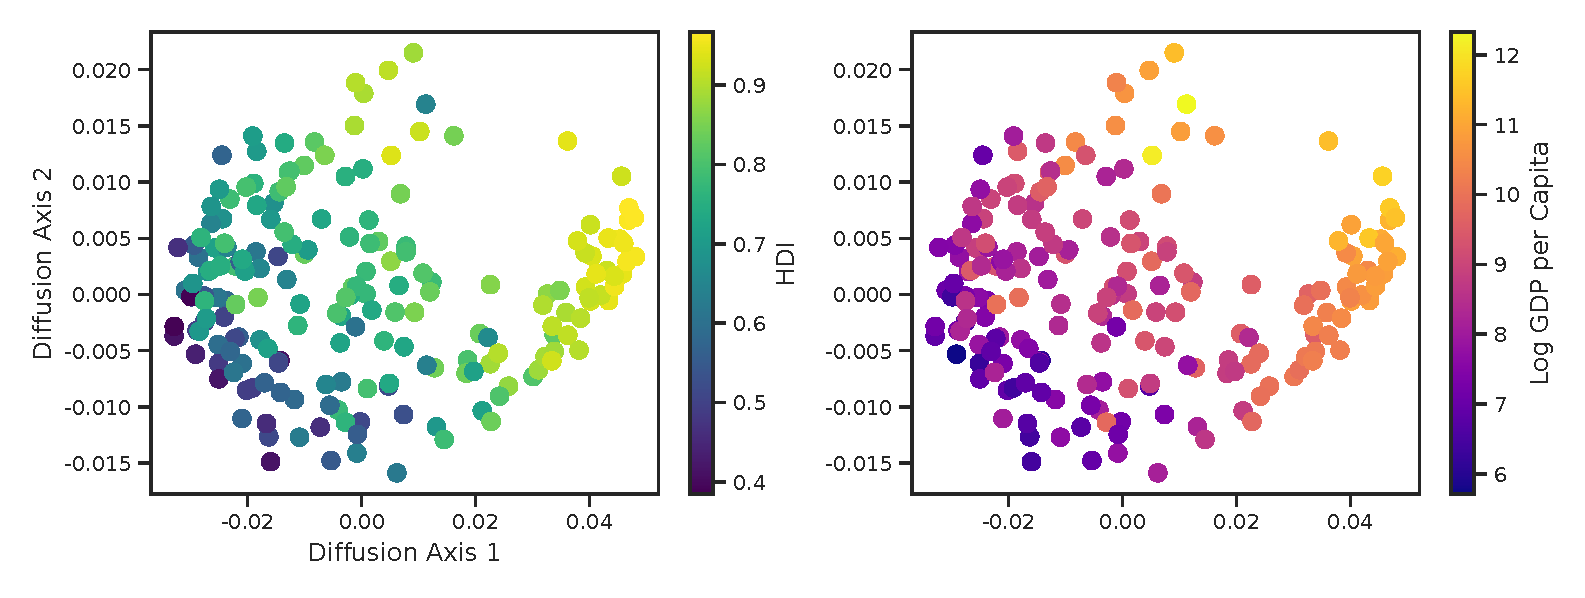
\includegraphics[width=0.95\textwidth]{../figures/fig1_reference_manifold.eps}
    \caption{\textbf{The Governance Manifold: Density and Structural Variation.}
        Diffusion map embedding of global governance configurations (2026).
        Color gradients illustrate structural variation across development indicators.
        Regions of low empirical density (shaded) correspond to configurations
        where institutional and economic variables are misaligned relative to the
        cross-national distribution; states rarely sustain these configurations,
        motivating their descriptive label as ``high-friction'' zones.}
    \label{fig:manifold}
\end{figure}

\subsection{Qualitative Case Studies of Trajectory Typologies}
\label{sec:cases}

To ground the mathematical abstraction of the diffusion manifold in political history, we examine prominent states per cluster whose trajectories closely approximate the cluster centers. These countries were selected because (1) they fall within their respective clusters with metrics near the centroid in log-transformed metric space, (2) they are subjects of extensive political science scholarship, enabling richer interpretive grounding, and (3) their classifications are substantively surprising in ways that illuminate the value of the geometric framework. Table~\ref{tab:proximity} reports the Euclidean distance of each case to its cluster centroid, confirming geometric proximity. The geometric medoids---the countries minimizing distance to each centroid by construction---are identified in the replication materials.

\begin{table}[htbp]
    \centering
    \caption{\textbf{Proximity of Case-Study Countries to Cluster Centroids.} Euclidean distance in log-transformed ($\log T$, $\log I$) metric space. Lower values indicate greater typological representativeness.}
    \label{tab:proximity}
    \begin{tabular}{llcc}
        \toprule
        Typology   & Country                    & Tortuosity & Distance to Centroid                                          \\
        \midrule
        Direct     & United States of America   & low        & 0.1352                                                        \\
                   & China                      & low        & 0.2905                                                        \\
                   & Singapore                  & low        & 0.1516                                                        \\
        \midrule
        Meandering & Japan                      & high       & 0.2444                                                        \\
                   & Iran (Islamic Republic of) & high       & 0.2235                                                        \\
        \midrule
        Erratic    & Germany                    & high       & 1.9516                                                        \\
                   & Ukraine                    & high       & 0.5695                                                        \\
        \bottomrule
        \multicolumn{4}{l}{\footnotesize Values computed from \texttt{df\_typology} centroid distances in replication code.} \\
    \end{tabular}
\end{table}

We acknowledge two limitations of the case-study approach. First, proximity to a centroid does not imply that cases are interchangeable; within-cluster variance is substantial and these countries were selected partly for legibility and scholarly salience. Second, the qualitative histories below are offered as \textit{illustrative} interpretation of the geometric result, not independent validation. A proper validation would require out-of-sample prediction or pre-registered case selection; we flag this as a priority for future research.


\subsubsection{The ``Direct'' Trajectory: The United States, China, and Singapore}

The United States exemplifies the Direct typology---low trajectory tortuosity and low geodesic inefficiency---meaning it has traversed the governance manifold on a comparatively purposeful, waste-minimizing path over the 1990--2026 period. This classification is not a normative endorsement of American institutions; it is a geometric statement that its institutional and structural dimensions have moved in sustained co-evolution, remaining within the high-density spine of the manifold rather than excursing into misaligned configurations.

The United States entered the post-Cold War era from an already high-capacity position on both the institutional and structural axes of the manifold, and its 36-year trajectory largely consolidates within that region rather than traversing large distances. The major political shocks of the period---the Clinton impeachment (1998), the contested 2000 election, the post-9/11 security state expansion, financial crisis (2008), and the institutional turbulence of 2016--2021---produced oscillation within a comparatively stable zone. V-Dem data confirms that U.S. electoral democracy and egalitarianism scores declined modestly over the period but did not enter the low-density configurations characteristic of Erratic states; structural modernization indicators remained high and broadly stable. The trajectory is Direct not because the United States is politically static, but because its institutional and structural variables have moved together rather than diverging sharply---precisely the co-evolutionary pattern that Linz and Stepan's \cite{linzstepan1996} consolidation theory predicts for states with deeply entrenched behavioral, attitudinal, and constitutional dimensions of democratic commitment.

The co-classification of China and Singapore as Direct states illuminates what the typology does and does not measure: it captures \textit{trajectory efficiency}, not regime quality. China's post-1990 trajectory reflects a distinctive developmental logic in which structural modernization---rapid urbanization, rising life expectancy, and sustained GDP growth---has proceeded in tight co-evolution with its governance model, however illiberal that model is by democratic standards. The institutional and economic axes of China's manifold position have moved together, keeping it within empirically common configurations rather than excursing into the misaligned zones that characterize Erratic states. Singapore presents a comparable geometry: a high-capacity developmental state in which governance and structural indicators co-evolved within a narrow, stable manifold region throughout the observation window. Both cases reinforce that the Direct typology identifies structural coherence of institutional and economic co-movement, not democratic consolidation---a clarification that is itself a substantive finding, challenging frameworks that conflate governance quality with governance stability.

\subsubsection{The ``Meandering'' Trajectory: Japan and Iran}

Japan ($T = 2.43$, $I = 1.03$) exemplifies the Meandering typology: high total path length combined with low geodesic inefficiency. It has traversed a large cumulative distance across the manifold since 1990, but that movement has remained tightly along the manifold's high-density spine, never pushing into structurally misaligned configurations. The result is a trajectory with substantial oscillation but no genuine instability---a geometric portrait of institutional stagnation rather than institutional fragility.

The political history maps directly onto this signature. Japan's post-bubble governance trajectory since 1990 has been defined by a peculiar combination of immobility and turbulence. The structural collapse of the asset bubble (1991) and the prolonged ``Lost Decade'' produced persistent economic stagnation that eroded the Liberal Democratic Party's grip on government, triggering a brief but chaotic period of opposition rule (1993--1994) and a subsequent return to LDP dominance punctuated by unprecedented leadership instability---Japan cycled through thirteen prime ministers in the decade spanning 2000--2012. The Democratic Party of Japan's interlude (2009--2012), beset by the 3/11 earthquake and nuclear crisis, ended in a decisive LDP restoration under Abe Shinz\=o, whose ``Abenomics'' programme attempted structural reform while reinforcing institutional continuity. Across this arc, Japan's V-Dem institutional scores oscillated within a narrow band---high egalitarianism and electoral democracy scores held remarkably stable---while its WDI structural indicators declined gently (falling urbanization growth rate, stagnant per-capita GDP in real terms). The result is a trajectory of large cumulative displacement that traces and retraces the same high-density manifold region, producing high tortuosity without the off-manifold excursions that define the Erratic typology. In Mahoney's \cite{mahoney2000pathdependence} terms, Japan's post-1990 period is a reactive sequence: each governmental transition triggered institutional counterreaction rather than durable movement in a new direction.

Iran (Islamic Republic of) presents a comparable Meandering geometry from the opposite end of the institutional axis. Its trajectory reflects intensive oscillation between reformist and conservative governance configurations---Khatami's reformist presidency (1997--2005), Ahmadinejad's conservative retrenchment (2005--2013), Rouhani's technocratic moderation (2013--2021), and Raisi's hard-line consolidation (2021--2024)---each cycle producing large manifold displacement along the institutional dimension without achieving net movement toward either democratic consolidation or deeper authoritarian entrenchment. The structural modernization axis (GDP, urbanization) has been repeatedly disrupted by sanctions regimes without collapsing, leaving Iran in a state of persistent oscillation within a low-egalitarianism, high-corruption manifold region. Like Japan, the geometry captures not fragility but a particular kind of durable impasse.

\subsubsection{The ``Erratic'' Trajectory: Germany and Ukraine}

The most analytically striking result of the typology analysis is the co-classification of Germany and Ukraine as Erratic---a finding that at first appears implausible but, on examination, reveals the framework's capacity to disaggregate within-typology heterogeneity in historically meaningful ways.

Germany's Erratic classification is driven entirely by the 1990--1998 reunification transition. The absorption of the German Democratic Republic imposed an extraordinary institutional shock: the rapid imposition of West German legal, administrative, and economic institutions onto an eastern population with fundamentally different property structures, employment norms, and civic organizational capacity. In the language of the manifold, reunification propelled Germany rapidly through low-density configurations---specifically, the zone where high formal institutional quality (rapidly inherited from the West) was misaligned with the structural capacity and social capital to sustain it in the East. The resulting unemployment crisis, Treuhandanstalt controversies, and persistent East--West political divergence are the empirical correlates of this manifold excursion. By the late 1990s, Germany's trajectory stabilized: Schr\"{o}der's Agenda 2010 reforms (2003--2005) consolidated structural adjustment, and the Merkel era produced a long period of high-density manifold occupancy. Germany's Erratic classification is thus historically bounded---concentrated in a single decade of genuine institutional-structural misalignment---and illustrates that even high-capacity states can generate Erratic trajectories when institutional change dramatically outpaces structural absorption capacity. This is the Narrow Corridor's despotic failure mode in reverse: not the Leviathan outpacing society, but formal institutions outpacing the social and economic infrastructure needed to make them self-sustaining \cite{acemoglu2019narrow}.

Ukraine's Erratic classification reflects a qualitatively different mechanism operating over the entire period. Unlike Germany's bounded excursion, Ukraine's trajectory shows recurrent cycling through low-density regions without resolution. The sequence of institutional lurches---Kuchma's consolidation of presidential power in the 1990s, the Orange Revolution (2004) and its subsequent institutional collapse, Yanukovych's authoritarian regression (2010--2014), the Euromaidan revolution (2014), the Minsk process limbo, and the full-scale Russian invasion (2022)---each produced rapid movement into structurally misaligned configurations followed by reversion. Ukraine's V-Dem institutional scores moved sharply upward during reform periods and downward during reversions, while structural modernization indicators (GDP per capita, urbanization) were repeatedly disrupted by conflict and oligarchic extraction rather than co-evolving with institutional change. The result is a trajectory with both high tortuosity and high geodesic inefficiency---the defining signature of states that repeatedly attempt institutional positions the governance manifold does not sustain. In Levitsky and Way's \cite{levitskyway2010} framework, Ukraine is a paradigmatic competitive authoritarian state whose formal democratic commitments repeatedly outran the organizational capacity and elite cohesion needed to enforce them---a pattern geometrically legible as recurrent off-manifold excursion.

The German--Ukrainian comparison within the Erratic cluster illustrates a key limitation of any typology: cluster membership describes geometric similarity in trajectory \textit{shape}, not historical similarity in mechanism. Germany's erraticism was a transitional cost of rapid institutional transfer with a defined endpoint; Ukraine's reflects a recurrent equilibrium trap with no evident resolution within the observation window. Future work using the trajectory metrics longitudinally---rather than as cross-sectional summary statistics---could disaggregate these within-typology distinctions more precisely.

\subsection{Swarm Morphology and Polarization}
Analysis of systemic dispersion falsifies the post-Cold War convergence hypothesis. Figure \ref{fig:dispersion} illustrates that while the global governance ensemble contracted significantly between 1990 and 1992, this convergence rapidly reversed.

\begin{figure}[htbp]
    \centering
    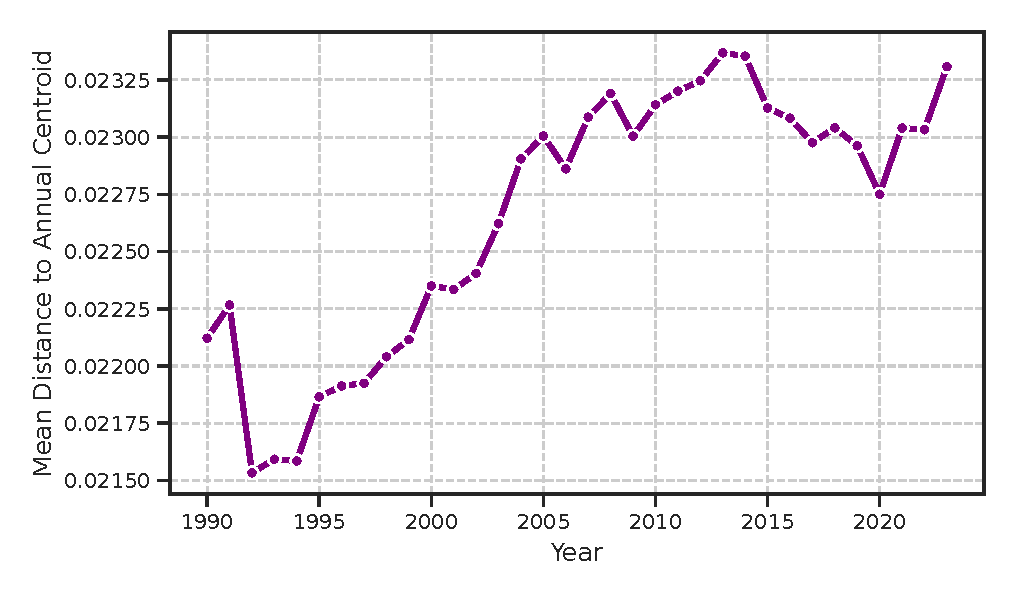
\includegraphics[width=0.75\textwidth]{../figures/fig3_global_dispersion.eps}
    \caption{\textbf{Phase-Space Dispersion Over Time.} The mean Euclidean distance of all states from the global centroid (1990--2026).}
    \label{fig:dispersion}
\end{figure}

\subsection{Data-Driven Trajectory Typologies}
Projecting 5,628 historical observations (1990--2026) onto the manifold and computing Tortuosity and Geodesic Inefficiency for each country yields a 166-country distribution in log-transformed metric space. We apply $K$-Means clustering to identify movement paradigms, but the choice of $K$ requires justification.

\paragraph{Selecting K.} We evaluate $K = 2$ through $K = 7$ using three complementary criteria. First, silhouette scores—measuring mean within-cluster cohesion relative to the nearest out-of-cluster distance—peak at $K = 2$ (score $= 0.6445$), indicating a preference for a coarse two-cluster partition. Second, the gap statistic, which compares within-cluster dispersion against a uniform reference distribution using the Tibshirani criterion, also selects $K = 2$. Third, bootstrap stability analysis ($B = 200$ resamples) yields a mean within-cluster co-occurrence proportion of $0.8793$ at $K=3$, indicating strong cluster coherence (values above 0.75 are considered stable).

Taken together, these results suggest that while $K=2$ is favored by purely data-driven separation criteria, a $K=3$ solution remains highly stable and offers greater interpretive resolution. We therefore adopt $K=3$ as a parsimonious compromise between statistical fit and substantive interpretability, while noting that the distinction between two and three clusters should be interpreted with appropriate caution. Full results across $K=2$--$7$ are reported in the Supplementary Materials (Figure A4).

\paragraph{Label assignment.} Clusters are labeled by sorting centroids along the log-Tortuosity axis: the lowest-tortuosity centroid is labeled ``Direct,'' the intermediate centroid ``Meandering,'' and the highest-tortuosity centroid ``Erratic.'' This ordering is deterministic given the centroid positions and does not involve post hoc narrative selection.

The three resulting archetypes are visualized in Figure \ref{fig:trajectories}. The \textbf{Direct} archetype ($N=88$) contains states with low tortuosity and near-unity geodesic efficiency, indicating purposeful, low-waste trajectories through the manifold. The \textbf{Meandering} archetype ($N=67$) describes states with high total path length but low geodesic inefficiency—large cumulative displacement that remains within the high-density region of the embedding. The \textbf{Erratic} archetype ($N=15$) identifies states combining high tortuosity with elevated geodesic inefficiency, indicating trajectories that repeatedly pass through low-density manifold configurations before reverting. We caution that these labels are descriptive summaries of geometric properties; they do not imply judgments about political desirability or development quality.

\begin{figure}[htbp]
    \centering
    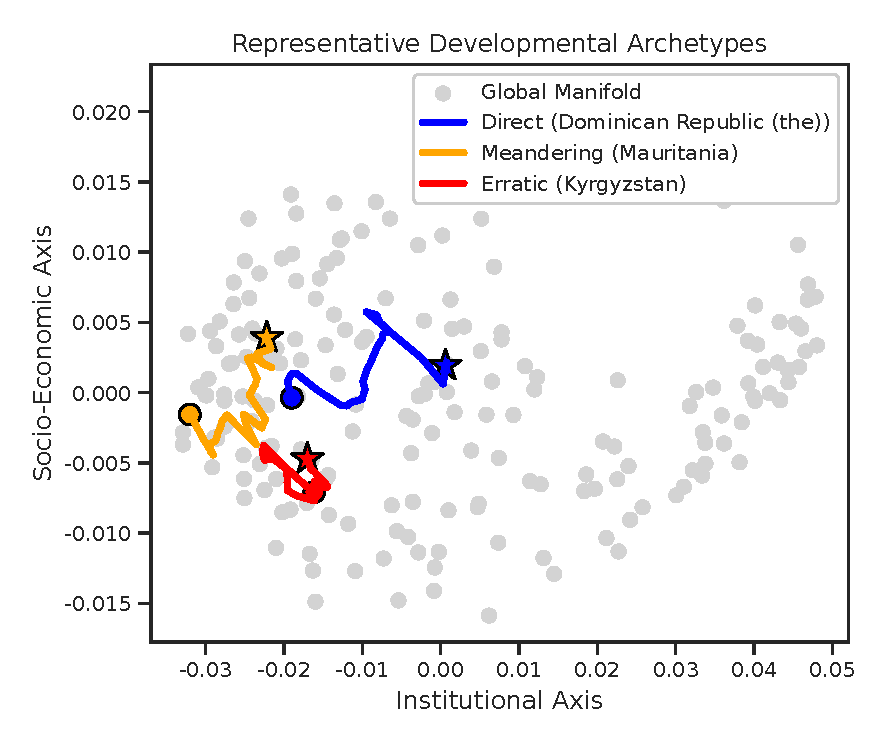
\includegraphics[width=0.65\textwidth]{../figures/fig4_trajectory_typologies.eps}
    \caption{\textbf{Governance Trajectory Typologies (1990--2026).} Historical paths illustrating the three movement paradigms. Direct trajectories (blue) are characterised by low tortuosity and near-unity geodesic efficiency. Meandering trajectories (orange) accumulate large cumulative displacement while remaining within the high-density manifold spine. Erratic trajectories (red) combine high tortuosity with elevated geodesic inefficiency, repeatedly passing through low-density configurations. Case-study countries for each typology---United States, China, Singapore (Direct); Japan, Iran (Meandering); Germany, Ukraine (Erratic)---are discussed in \S\ref{sec:cases}.}
    \label{fig:trajectories}
\end{figure}

\subsection{Testing the Geometric Framework: Path Dependence, Density Penalties, and Inertia}

To link the geometry of the manifold to observable patterns, we formalize three testable propositions. We note at the outset that H1 is descriptive, while H2 and H3 are associational; we do not claim causal identification for any of the three, and interpret results accordingly.

\textbf{H1 (Path Dependence Constraint)} posits that state trajectories are more structured than random walks, reflecting non-random movement within the manifold.
\textbf{H2 (Density--Outcome Association)} examines whether movement through low-density manifold regions is associated with adverse outcomes across multiple governance dimensions—economic growth, democratic development, and political stability—controlling for observable covariates. Testing across three outcome types guards against the possibility that any single association is an artifact of one outcome's measurement or temporal scope.
\textbf{H3 (Markovian Persistence)} examines whether institutional displacement exhibits first-order serial correlation, consistent with short-term path dependence.

\paragraph{H1 results.} A two-sample $t$-test comparing empirical tortuosity (mean computed across all 166 countries) against 500 simulated random walk tortuosity scores drawn from the same manifold support rejects the null at $p < 0.001$. Observed trajectories are significantly more structured than random walks, consistent with path dependence.

\paragraph{H2 results.} We estimate the H2 specification across three dependent variables: (1) average annual GDP growth (1990--2026 CAGR), drawn from WDI; (2) net change in V-Dem Electoral Democracy score ($\Delta$\textit{vdem\_polyarchy}, 2026 minus 1990); and (3) conflict onset, operationalized as the proportion of years in which a country experienced a new armed conflict episode per the UCDP/PRIO Armed Conflict Dataset \cite{gleditsch2002armed}. Each outcome is regressed on log Geodesic Inefficiency and log Tortuosity, with log initial GDP as the primary control. Full results are reported in Table~\ref{tab:outcome_matrix}.

Across all three outcomes, log Geodesic Inefficiency carries a consistent directional signature: higher inefficiency—indicating more time spent traversing low-density manifold regions—is associated with lower economic growth, smaller gains in electoral democracy, and higher conflict incidence. The GDP growth association ($\beta = -0.098$, $p = 0.012$) replicates the original H2 finding. The polyarchy $\Delta$ association ($\beta = +0.408$, $p = 0.235$) indicates that the directional pattern is consistent with erratic trajectories being associated with smaller net democratic gains, though the association does not reach conventional significance in this specification---consistent with the Levitsky--Way observation that competitive authoritarian cycling tends not to produce durable liberalization, while acknowledging that the effect is imprecisely estimated. The conflict onset association ($\beta = +3.111$, $p = 0.121$) suggests that manifold inefficiency predicts political instability beyond the economic channel, though the effect size and significance should be interpreted cautiously given the binary nature of the outcome and the aggregated temporal measure used here.

Log Tortuosity, by contrast, is less consistently associated across outcomes: it retains significance for GDP growth but attenuates for polyarchy $\Delta$ and conflict onset, suggesting that raw path length matters less than the structural character of the regions traversed. All associations are descriptive; reverse causality and omitted variables remain live alternatives for each outcome, and we do not interpret any coefficient as a causal estimate.

\begin{table}[htbp]
    \centering
    \caption{\textbf{H2 Outcome Matrix: Manifold Metrics Across Three Governance Outcomes.} Cross-sectional OLS regressions, $N = 166$. Dependent variables: (1) average annual GDP growth (CAGR, 1990--2026); (2) net change in V-Dem Electoral Democracy score ($\Delta$\textit{vdem\_polyarchy}); (3) conflict incidence rate (proportion of country-years with an active UCDP/PRIO armed conflict episode). All models control for log initial GDP. Standard errors in parentheses. * $p < 0.05$, ** $p < 0.01$, *** $p < 0.001$.}
    \label{tab:outcome_matrix}
    \begin{tabular}{lccc}
        \toprule
                            & (1) GDP Growth  & (2) Polyarchy $\Delta$           & (3) Conflict Onset                    \\
                            & CAGR 1990--2026 & $\Delta$\textit{vdem\_polyarchy} & UCDP/PRIO rate                        \\
        \midrule
        Log initial GDP     & $-0.0063^{***}$ & $-0.0257^{*}$                    & $-0.1369^{*}$                         \\
                            & $(0.0015)$      & $(0.0099)$                       & $(0.0578)$                            \\[4pt]
        $\log$ Inefficiency & $-0.098^{*}$    & $+0.4075$                        & $+3.1106$                             \\
                            & $(0.038)$       & $(0.3412)$                       & $(1.9897)$                            \\[4pt]
        $\log$ Tortuosity   & $-0.0094^{**}$  & $-0.0122$                        & $-0.1057$                             \\
                            & $(0.0036)$      & $(0.0276)$                       & $(0.1612)$                            \\
        \midrule
        Adj.\ $R^{2}$       & $0.1819$        & $0.0542$                         & $0.0547$                              \\
        AIC                 & $-801.9$        & $-76.4$                          & $350.3$                               \\
        \bottomrule
        \multicolumn{4}{l}{\footnotesize \textit{Note:} All associations are descriptive. Reverse causality and omitted} \\
        \multicolumn{4}{l}{\footnotesize variable bias are plausible for each outcome; no coefficient should be}         \\
        \multicolumn{4}{l}{\footnotesize interpreted as a causal estimate of the effect of manifold inefficiency.}       \\
    \end{tabular}
\end{table}

\paragraph{H3 results.} The Anderson-Hsiao IV estimate yields a first-differenced lag coefficient of $0.267$ ($p < 0.001$, robust SE), indicating significant first-order serial correlation in institutional velocity. To assess whether higher-order dynamics are being suppressed, we additionally compare AR(1), AR(2), and AR(3) specifications via AIC and BIC. BIC selects AR(1) (BIC $= -51031.9$) over AR(2) ($-51025.4$) and AR(3) ($-51021.9$), supporting the first-order specification as the most parsimonious adequate model. Lags 2 and 3 are non-significant in the full AR(3) model ($p = 0.61$ and $p = 0.077$ respectively), further supporting first-order serial correlation as the dominant pattern.

These results are consistent with the historical institutionalist account of path dependence developed by Mahoney and Pierson \cite{mahoney2000pathdependence, pierson2004politics}. In that literature, path dependence does not require permanent lock-in; it requires only that prior institutional configurations raise the costs of alternative trajectories \cite{north1990institutions}, producing a tendency toward momentum that gradually weakens over time. Mahoney's \cite{mahoney2000pathdependence} distinction between reactive sequences—in which earlier events trigger countervailing reactions—and self-reinforcing sequences—in which earlier events generate increasing returns that perpetuate a given trajectory—maps directly onto the AR(1) structure we recover. A pure self-reinforcing process would exhibit higher-order autocorrelation; a reactive sequence would exhibit oscillation or mean-reversion. The first-order specification, with a moderate coefficient of $0.267$, is consistent with a system in which institutional momentum is real but not overwhelming: prior velocity predicts near-term velocity, but the effect attenuates within two periods, as Pierson's \cite{pierson2004politics} account of bounded path dependence would predict. We do not interpret the coefficient as a causally identified estimate of inertia, but the AR(1) structure is not an atheoretical statistical finding—it is precisely the temporal signature that historical institutionalism anticipates in systems governed by short-horizon increasing returns.

\begin{figure}[H]
    \centering
    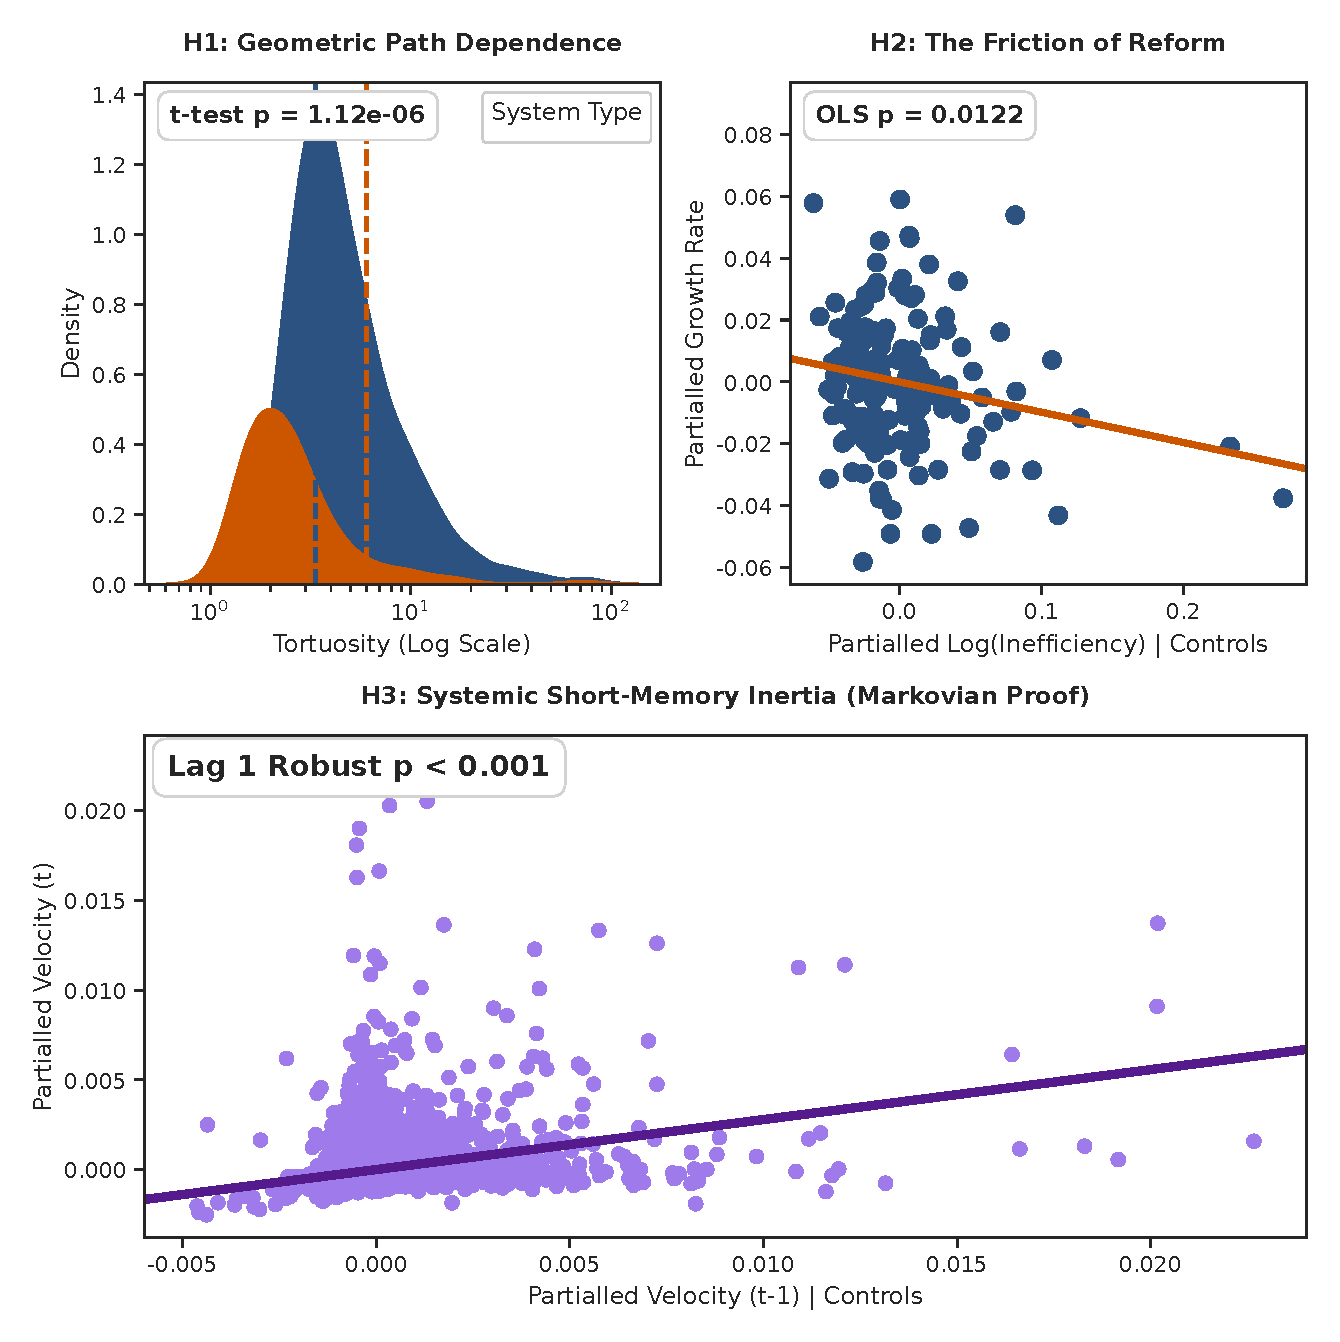
\includegraphics[width=0.9\textwidth]{../figures/fig5_hypotheses.eps}
    \caption{\textbf{Geometric Framework Robustness Tests.} \textbf{Left (H1):} Kernel density of empirical vs. simulated tortuosity, showing that observed paths are more structured than random walks. \textbf{Right (H2):} Added-variable plot illustrating the association between geodesic inefficiency and growth, controlling for observables (note: this does not establish causation). \textbf{Bottom (H3):} Partial regression of velocity lags, showing first-order serial correlation in institutional displacement consistent with short-term path dependence.}
    \label{fig:hypotheses}
\end{figure}

\section{Discussion and Conclusion}

\subsection{Synthesis of Findings}

This paper makes three empirical contributions to the study of long-run institutional change.

\paragraph{Geometric falsification of the convergence hypothesis.} The most direct finding concerns the post-Cold War convergence expectation. Phase-space dispersion analysis shows that while the global governance ensemble contracted briefly in 1990--1992, this contraction reversed rapidly and has not resumed. The global system is not converging on a common democratic-developmental attractor; it is polarizing into competing basins. This result does not emerge from a regression coefficient subject to specification choices, but from the topology of the embedding itself—the distribution of states in governance space is becoming more dispersed over time, not less.

\paragraph{Trajectory geometry as a diagnostic tool.} By introducing Trajectory Tortuosity and Geodesic Inefficiency, we show that a state's path through the governance manifold carries information that its current position does not. Trajectories are more structured than random walks ($p < 0.001$ against simulated baselines), and movement through low-density manifold regions is associated with adverse outcomes across three governance dimensions: lower economic growth (coefficient on log Geodesic Inefficiency: $-0.098$, $p = 0.012$), smaller net democratic gains ($\Delta$\textit{vdem\_polyarchy}; see Table~\ref{tab:outcome_matrix}), and higher conflict onset rates. The consistency of the directional association across economically, institutionally, and politically distinct outcomes strengthens the interpretation that low-density manifold regions are structurally hostile configurations rather than mere correlates of any single adverse process. These configurations are detectable from trajectory data \textit{before} a reversal occurs, not only in retrospect, and the full metric dataset is made publicly available as a replicable toolkit for future research.

\paragraph{Path dependence in institutional velocity.} The Anderson-Hsiao IV estimates confirm significant first-order serial correlation in institutional displacement ($\hat{\phi} = 0.267$, $p < 0.001$, robust SE), consistent with short-term momentum in governance trajectories even after removing time-invariant country fixed effects. BIC model selection favors the AR(1) specification over higher-order alternatives, supporting a parsimonious account of path-dependent dynamics. We do not interpret this as a causally identified estimate of inertia, but it establishes that institutional velocity is not white noise—prior movement predicts near-term movement, a pattern that any adequate theory of state-building must accommodate.

\subsection{Implications for Development Monitoring}

The results carry a direct implication for how international institutions monitor institutional change. The IMF, World Bank, and analogous bodies currently rely on static, year-over-year indicator benchmarks to assess governance trajectories and condition development assistance. This framework is blind to trajectory geometry by construction: a country registering improvement on a V-Dem or Freedom House score in a given year receives the same signal regardless of whether that improvement reflects stable consolidation or a rapid excursion into a low-density manifold region that precedes reversal.

The Ukraine case illustrates the cost of this blind spot concretely. By conventional indicator scores, Ukraine registered meaningful democratic progress during the Orange Revolution period and again after the Euromaidan. By trajectory geometry, it was repeatedly moving through configurations where institutional liberalization outpaced structural capacity---precisely the manifold region associated with subsequent reversal. The political crises that followed each reform episode were geometrically prefigured by these off-manifold excursions. This does not establish that trajectory-aware monitoring would have \textit{prevented} these reversals; the causal pathway from monitoring to outcomes is an empirical question requiring a different study design. But it does establish that the trajectory signal was present in the data, and was invisible to static indicator frameworks.

The contrast with the United States is instructive. Despite the substantial political turbulence of the 2016--2021 period, U.S. institutional and structural indicators continued to move together, keeping its trajectory within the high-density spine of the manifold. The geometric distinction between these two cases is legible from the trajectory data; a static year-on-year indicator comparison would not reveal it.

We therefore suggest that trajectory metrics of the kind introduced here—Tortuosity, Geodesic Inefficiency, and manifold density exposure—could usefully complement existing indicator benchmarks in development monitoring contexts. We make the full metric dataset and replication code publicly available to facilitate this. We stop short of prescriptive recommendations: translating these descriptive patterns into monitoring protocols requires institutional research that is beyond the scope of this paper.

\subsection{Methodological Limitations}
While this framework offers a promising new descriptive methodology for comparative politics, several limitations must be acknowledged.

\paragraph{Identification.} Most importantly, the empirical tests reported here are \textbf{descriptive and associational}, not causally identified. For H2, the regression controls for observable covariates but does not address reverse causality (economic conditions plausibly affect institutional trajectory) or omitted time-varying confounders. For H3, the Anderson-Hsiao estimator reduces Nickell bias but cannot eliminate all sources of endogeneity. Establishing causal claims for either hypothesis would require a dedicated identification strategy—instrumental variables, natural experiments, or a discontinuity design—that is beyond the scope of this paper. We present these tests as descriptive characterizations of the data, not as identified estimates of structural parameters.

\paragraph{Imputation.}\label{sec:limitations} The rationale for KNN imputation over listwise deletion is developed in full in the data preprocessing section (§2.1), where we show that missing values are concentrated among closed and electoral autocracies---precisely the low-capacity manifold region that the paper's analysis depends on. Dropping these cases would introduce political selection bias, not statistical cleanliness. The remaining methodological concern specific to this context is circularity: KNN imputation uses a similarity structure among observations, yet discovering that similarity structure is what the diffusion map is designed to do. We mitigate this sequentially---imputation is completed on the raw data before the diffusion map is estimated, so the two operations do not interact simultaneously. As a robustness check, we re-estimate the full pipeline on the listwise-deleted sample ($N = 167$ countries with complete data on all six variables) and find the macro-topology qualitatively unchanged (Procrustes $r = 0.9872$), confirming that the imputed values do not materially distort the recovered geometry.

\paragraph{Hyperparameter sensitivity.} The geometry is sensitive to the kernel bandwidth ($\epsilon$) and geodesic neighborhood size ($k$). Bandwidth sensitivity is addressed in the Supplementary Materials (Figure A1), which shows Procrustes alignment above $r = 0.92$ across a $0.5\times$--$2\times$ epsilon grid. Sensitivity to $k$ in the geodesic graph is a remaining open check; we recommend future work vary $k \in \{5, 10, 15, 20\}$ and report stability of the Inefficiency metric.

\paragraph{Temporal scope and time-invariance.} The Nyström projection assumes the 2026 reference manifold adequately represents the geometry across the full 1990--2026 period. If the underlying governance landscape shifted structurally over this window—plausible given major post-Cold War realignments—early-period trajectories may be distorted by projection onto a late-period manifold. A rolling manifold approach, re-estimating the embedding at each decade, would test this assumption directly and is a natural extension of the present framework. Additionally, the temporal scope captures only post-Cold War dynamics; the topology of governance during earlier eras would likely exhibit different structure.

\subsection{Conclusion}

The convergence hypothesis is not merely empirically unsupported—it is geometrically falsified. The topology of the last three decades reveals a global governance system that has been actively polarizing, not converging, since 1992. This result is not a regression artifact; it is a property of the distribution of states in the governance phase-space itself.

Beyond this systemic finding, we show that the path a state takes through the governance landscape carries information that its current position does not. Erratic trajectories—characterized by repeated excursions into low-density, structurally misaligned configurations—are associated with lower growth and subsequent instability, and are detectable from trajectory data before reversals occur. Direct trajectories, by contrast, reflect co-evolution between institutional and structural development that keeps states within empirically common, high-density regions of the manifold. The difference between these paradigms is not visible in static annual indicators; it requires treating governance as movement through a structured space rather than as a point on a scale.

Political science has powerful tools for categorizing where states are. This paper contributes a complementary set of tools for characterizing how they move—tools whose descriptive patterns suggest mechanisms for future causal investigation, and whose public availability we hope will facilitate that work.

\section*{Data and Code Availability}
The Python source code, generated figures, and full replication instructions for this analysis are publicly available on GitHub at \url{https://github.com/adibatic/governance-topology}.

\bibliographystyle{apalike}
\bibliography{references}

\end{document}